\documentclass[tikz,border=10pt]{standalone}
\usepackage{tikz}
\usetikzlibrary{positioning}
\usepackage{tikz-feynman}
\begin{document}

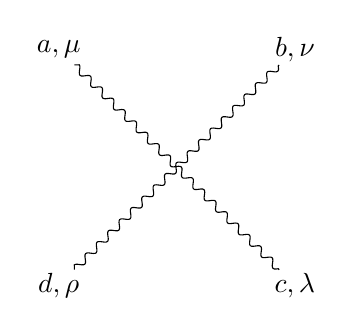
\begin{tikzpicture}[baseline]
    \begin{feynman}
        %% fig a
        \vertex[dot] (a1) at (0,0);
        \vertex[above right =1.3 and 1.3  of a1] (a2); % 右上
        \node [above right =1.5 and 1.5  of a1,anchor=center] {$b, \nu$};
        \vertex[above right =-1.3 and 1.3  of a1] (a3); %左上
        \node [above right =-1.5 and 1.5  of a1,anchor=center] {$c, \lambda$};
        \vertex[above right =1.3 and -1.3  of a1] (a4); % 右下
        \node [above right =1.5 and -1.5  of a1,anchor=center] {$a, \mu$};
        \vertex[above right =-1.3 and -1.3  of a1] (a5); %左下
        \node [above right =-1.5 and -1.5  of a1,anchor=center] {$d, \rho$};
        % 对各个顶点连线
        \diagram*{
            { [edge=photon]	(a2) --  (a5),(a3) --  (a4),
                },
        };
    \end{feynman}
\end{tikzpicture}

\end{document}